\begin{figure}
\pgfplotstableread[col sep=comma]{pgf-speedup-figs/results/cover_homology/clique.11.22720.csv}\tablecovermblb
\pgfplotstableread[col sep=comma]{pgf-speedup-figs/results/concurrent_homology/clique.11.22720.csv}\tableconcurrentmblb
\pgfplotstableread[col sep=comma]{pgf-speedup-figs/results/phat_14_chunk/clique.11.22720.csv}\tablephatchunkmblb
\pgfplotstableread[col sep=comma]{pgf-speedup-figs/results/phat_14_ss/clique.11.22720.csv}\tablephatssmblb
%%compute first regression 
\pgfplotstablecreatecol[linear regression={x=num_threads, y=speedup}]{regression}{\tablecovermblb}
\xdef\slopeA{\pgfplotstableregressiona} 
\xdef\interceptA{\pgfplotstableregressionb}
%%compute second regression 
\pgfplotstablecreatecol[linear regression={x=num_threads, y=speedup}]{regression}{\tableconcurrentmblb}
\xdef\slopeB{\pgfplotstableregressiona} 
\xdef\interceptB{\pgfplotstableregressionb}
%%make percentages
\pgfmathparse{\slopeA*100}
\pgfmathprintnumberto[precision=0]{\pgfmathresult}{\efficiencyA}
\pgfmathparse{\slopeB*100}
\pgfmathprintnumberto[precision=0]{\pgfmathresult}{\efficiencyB}
%\fbox{
\begin{subfigure}[t]{.45\linewidth}
\begin{tikzpicture}[scale=1]
\begin{axis}[legend cell align=left,xlabel=\# of threads, ylabel=speedup factor, minor y tick num={3}, minor x tick num={1},legend style={legend pos=north west, font=\tiny}]
\legend{$\proc{Multicore-Homology}$,  $\proc{Heuristic-MH}$, $\proc{Chunk}$~\cite{bkr-cccph-13}, $\proc{Spectral-Sequence}$~\cite{bkr-cccph-13}, ideal}
\addplot table [x=num_threads, y=speedup, col sep=comma, skip coords between index={0}{1}] from  {\tableconcurrentmblb};
\addplot table [x=num_partitions, y=speedup, col sep=comma, skip coords between index={0}{1}] from {\tablecovermblb};
\addlegendentry{Heuristic \mv{}} %
\addplot table [x=num_partitions, y=speedup, col sep=comma, skip coords between index={0}{1}] from {\tablephatchunkmblb}; 
\addplot table [x=num_partitions, y=speedup, col sep=comma, skip coords between index={0}{1}] from {\tablephatssmblb};
\addplot[dash pattern=on 4pt off 1pt on 4pt off 4pt, domain=2:11]{x};
\addlegendentry{ideal speedup}
\end{axis}
\end{tikzpicture}
\caption{We achieve ${\sim}\efficiencyA$\% efficiency across 11 cores via \proc{Heuristic-MH} and ${\sim}\efficiencyB\%$ via \proc{Multicore-Homology}. 
We also plot the speedup factor of the parallel algorithms \proc{Chunk} and \proc{Spectral-Sequence} from Bauer et. al~\cite{bkr-cccph-13}.}
\label{fig:blobs-speedup}
\end{subfigure}
%}
\hspace{1cm}
%\fbox{
\begin{subfigure}[t]{.45\linewidth}
\vspace{-1.27cm}
\begin{tikzpicture}[scale=1]
\fbox{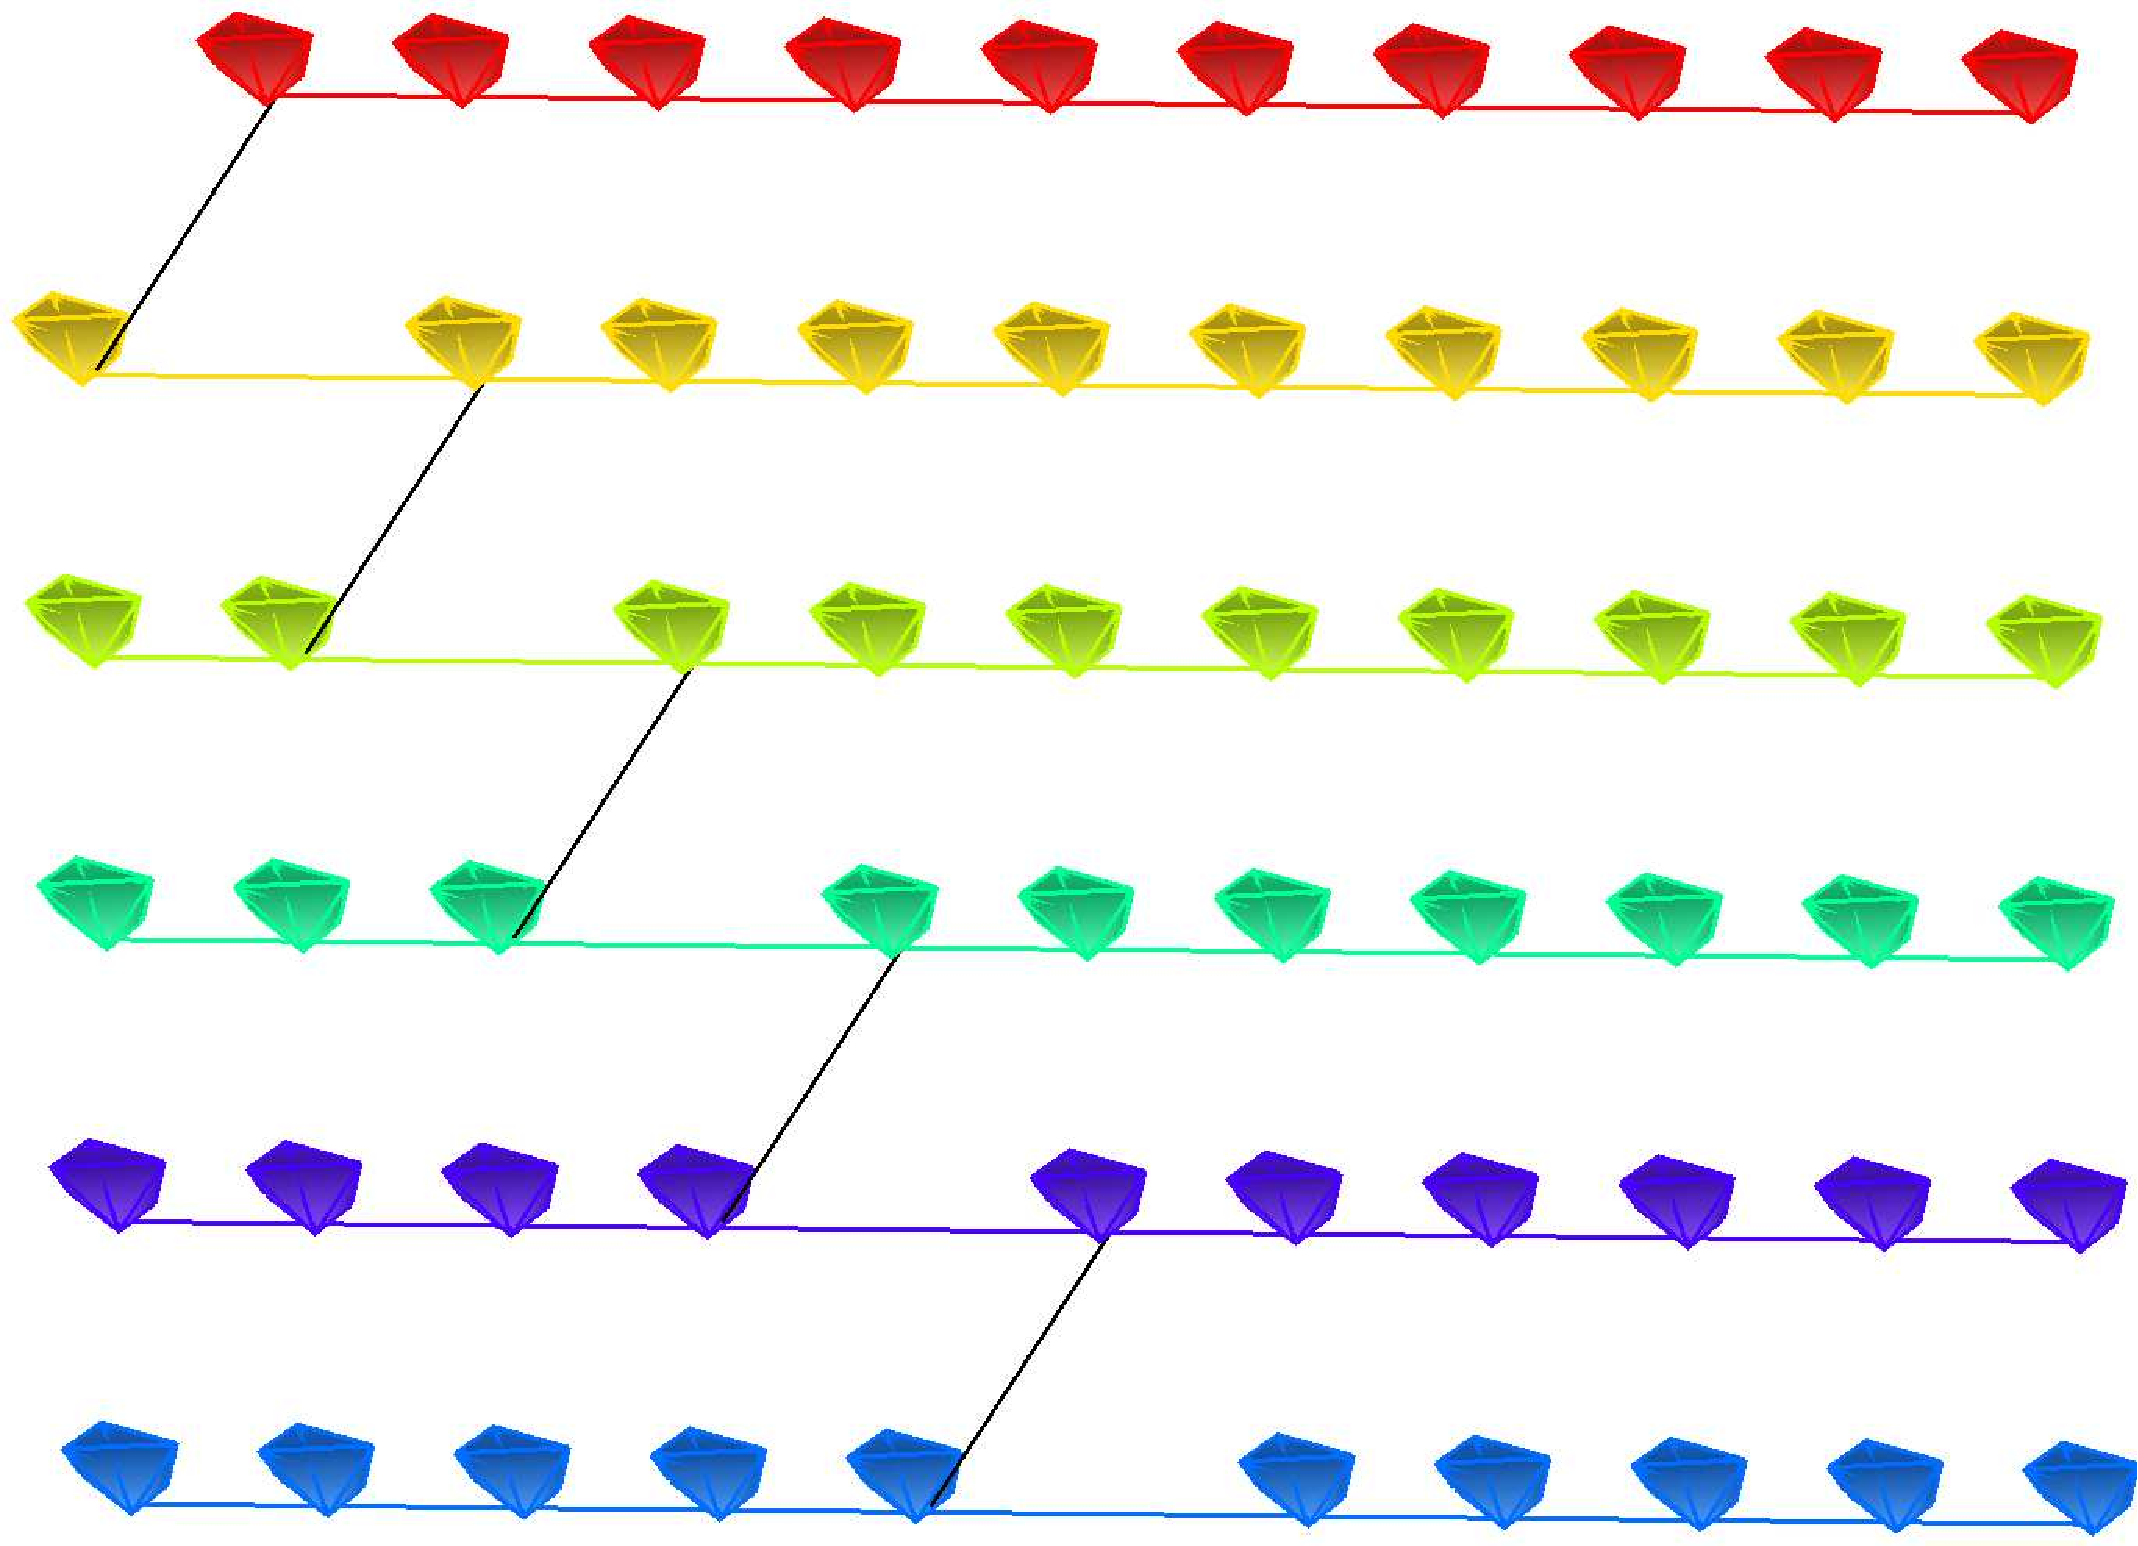
\includegraphics[width=.98\linewidth]{blobs-vis}\vspace{1cm}}
\end{tikzpicture}
\vspace{1cm}
\caption{Shown is a portion of the simply connected input space $\multiblob$. {\blobs} contains ${\sim}22$K copies of a fully connected 10 dimensional complex on 11 vertices each connected to the next by a single edge.
Each color represents a portion of 7 sets of a cover by 12 pieces.}
\label{fig:blobs-vis}
\vspace*{\baselineskip}
\end{subfigure}
%}
\caption{On the left is the speedup in homology computation for the 10 dimensional complex with 45M simplices partially shown on the right.}
\label{fig:front-picture}
\end{figure}